\documentclass[sigconf]{acmart}

\usepackage{listings}
\usepackage{booktabs}
\usepackage{graphicx}

% Copyright
%\setcopyright{none}
%\setcopyright{acmcopyright}
%\setcopyright{acmlicensed}
\setcopyright{rightsretained}
%\setcopyright{usgov}
%\setcopyright{usgovmixed}
%\setcopyright{cagov}
%\setcopyright{cagovmixed}

%% Comments
\newif\ifcomments\commentstrue

\ifcomments
\newcommand{\authornt}[3]{\textcolor{#1}{[#3 ---#2]}}
\newcommand{\todo}[1]{\textcolor{red}{[TODO: #1]}}
\else
\newcommand{\authornt}[3]{}
\newcommand{\todo}[1]{}
\fi

\newcommand{\ds}[1]{\authornt{red}{MSN}{#1}} %Dan
\newcommand{\wss}[1]{\authornt{blue}{SS}{#1}} %Spencer
\newcommand{\jc}[1]{\authornt{magenta}{MSN}{#1}} %Jacques
\newcommand{\spr}[1]{\authornt{green}{AW}{#1}} %Steven

% DOI
%\acmDOI{10.475/123_4}

% ISBN
%\acmISBN{123-4567-24-567/08/06}

%Conference
\acmConference[SE-CSE\_SE-CoDeSE]{2017 International Workshop on Software Engineering
  for High Performance Computing in Computational and Data-Enabled Science and
  Engineering}{November 2017}{Denver, Colorado, USA} 
\acmYear{2017}
\copyrightyear{2017}

%\acmPrice{15.00}

\begin{document}
\title{Progress Report on Drasil: A Framework for Scientific Knowledge Capture and Artifact Generation}
% \titlenote{Produces the permission block, and
%   copyright information}
% \subtitle{Extended Abstract}
% \subtitlenote{The full version of the author's guide is available as
%   \texttt{acmart.pdf} document}

\author{Daniel Szymczak}
% \authornote{Dr.~Trovato insisted his name be first.}
% \orcid{1234-5678-9012}
\affiliation{%
  \institution{Computing and Software Department, McMaster University}
  \streetaddress{1280 Main Street West}
  \city{Hamilton} 
  \state{Ontario} 
  \postcode{L8S 4K1}
}
\email{szymczdm@mcmaster.ca}

\author{Spencer Smith}
% \authornote{Dr.~Trovato insisted his name be first.}
% \orcid{1234-5678-9012}
\affiliation{%
  \institution{Computing and Software Department, McMaster University}
  \streetaddress{1280 Main Street West}
  \city{Hamilton} 
  \state{Ontario} 
  \postcode{L8S 4K1}
}
\email{smiths@mcmaster.ca}

\author{Jacques Carette}
% \authornote{Dr.~Trovato insisted his name be first.}
% \orcid{1234-5678-9012}
\affiliation{%
  \institution{Computing and Software Department, McMaster University}
  \streetaddress{1280 Main Street West}
  \city{Hamilton} 
  \state{Ontario} 
  \postcode{L8S 4K1}
}
\email{carette@mcmaster.ca}

\author{Steven Palmer}
%\authornote{The secretary disavows any knowledge of this author's actions.}
\affiliation{%
  \institution{Computing and Software Department, McMaster University}
  \streetaddress{1280 Main Street West}
  \city{Hamilton} 
  \state{Ontario} 
  \postcode{L8S 4K1}
}
\email{palmes4@mcmaster.ca}

% The default list of authors is too long for headers}
% \renewcommand{\shortauthors}{B. Trovato et al.}

\begin{abstract}
abstract here
\end{abstract}

%
% The code below should be generated by the tool at
% http://dl.acm.org/ccs.cfm
% Please copy and paste the code instead of the example below. 
%
 \begin{CCSXML}
<ccs2012>
<concept>
<concept_id>10002950.10003705</concept_id>
<concept_desc>Mathematics of computing~Mathematical software</concept_desc>
<concept_significance>300</concept_significance>
</concept>
<concept>
<concept_id>10011007.10011074.10011092</concept_id>
<concept_desc>Software and its engineering~Software development techniques</concept_desc>
<concept_significance>300</concept_significance>
</concept>
<concept>
<concept_id>10011007.10011074.10011092.10011782</concept_id>
<concept_desc>Software and its engineering~Automatic programming</concept_desc>
<concept_significance>300</concept_significance>
</concept>
</ccs2012>
\end{CCSXML}

\ccsdesc[300]{Mathematics of computing~Mathematical software}
\ccsdesc[300]{Software and its engineering~Software development techniques}
\ccsdesc[300]{Software and its engineering~Automatic programming}

\keywords{scientific computing, software quality, software engineering, document
driven design, code generation}

\maketitle

\section{Introduction} \label{SecIntroduction}

- goal to improve the quality of Scientific Computing Software (SCS)
- in particular the qualities of certifiability, reusability and reproducibility
for large multi-year, multi-developer projects where the end users do much of
the development
- especially important to improve quality where correctness impacts safety
- examples of nuclear safety analysis and medical imaging

- improved documentation is an important part of improved quality, but too much
time and effort for SCS developers, especially when they are often dealing with
rapid change.  SCS developers tend to dislike documentation. As observed by
  Carver~\cite{CarverEtAl2007}, scientists do not view rigid, process-heavy
  approaches, favourably.  Moreover, they often consider reports for each stage
  of software development as counterproductive~\cite[p.~373]{Roache1998}.

\begin{itemize}
\item Documentation provides advantages
\begin{itemize}
\item Improves verifiability, reusability, reproducibility, etc.
\item From \cite{Parnas2010}
\begin{itemize}
\item easier reuse of old designs
\item better communication about requirements
\item more
  useful design reviews
\item etc.
% \item easier integration of separately written modules, more
%   effective code inspection, more effective testing, and more efficient
%   corrections and improvements
\end{itemize}
\item New doc found 27 errors \citep{SmithAndKoothoor2016}
\item Developers see advantage \cite{SmithJegatheesanAndKelly2016}
\end{itemize}
\item But documentation is felt to be ...
\begin{itemize}
\item Too long
\item Too difficult to maintain
\item Not amenable to change
\item Too tied to waterfall process
\item Reports counterproductive \citep{Roache1998}
\end{itemize}
\item {\textbf{The Solution?}}
\end{itemize}

Drasil - a solution proposed in a position paper~\cite{SzymczakEtAl2016} - capture the scientific and documentation knowledge
and then generate the code and other software artifacts

- work on Drasil has continued since the position paper, as described below -
provide a roadmap of the paper

\section{Design of Drasil} \label{SecDevProcess}

- an overview, with an emphasis on the notion of chunks would be good - should
mention which DSLs are part of DSL - maybe the ontology figure?
- should mention GOOL

\begin{figure}[htpb]
\centering
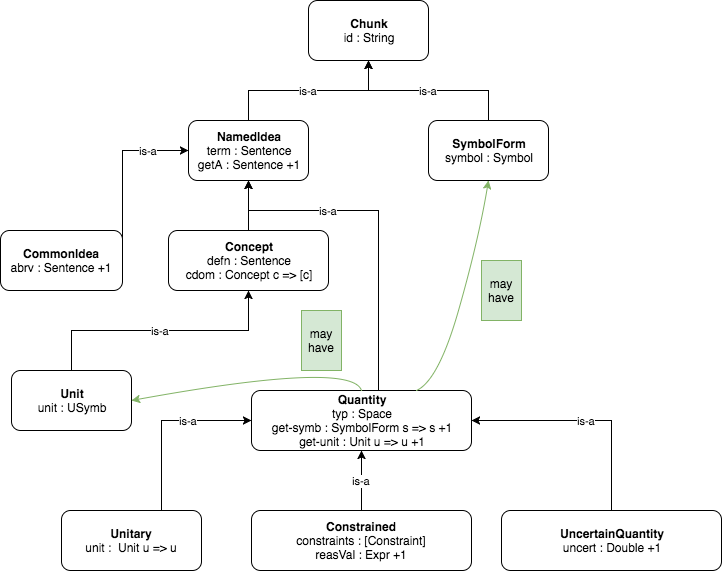
\includegraphics[width=0.5\textwidth]{figures/class_hierarchy.png}
\caption{Relationships Between Drasil Classes}
\label{element}
\end{figure}

\section{Development Process for Drasil} \label{SecDevProcess}

- concurrent development of 5 different examples - list the examples - mention
that they overlap with~\cite{SmithJegatheesanAndKelly2016}
- use of GitHub
- peer review of code
- issue tracking
- refactoring - finding patterns
- knowledge extraction
- reduction of duplication

\section{GlassBR Example} \label{SecGlassBR}

- introduce example from Civil Engineering - say what the inputs are to GlassBR
and what it calculates
- bottom up approach to presentation - start with chunks, build up to SRS, traceability

- start with data definition for Jtol generated by Drasil

\begin{figure}[htpb]
\begin{center}
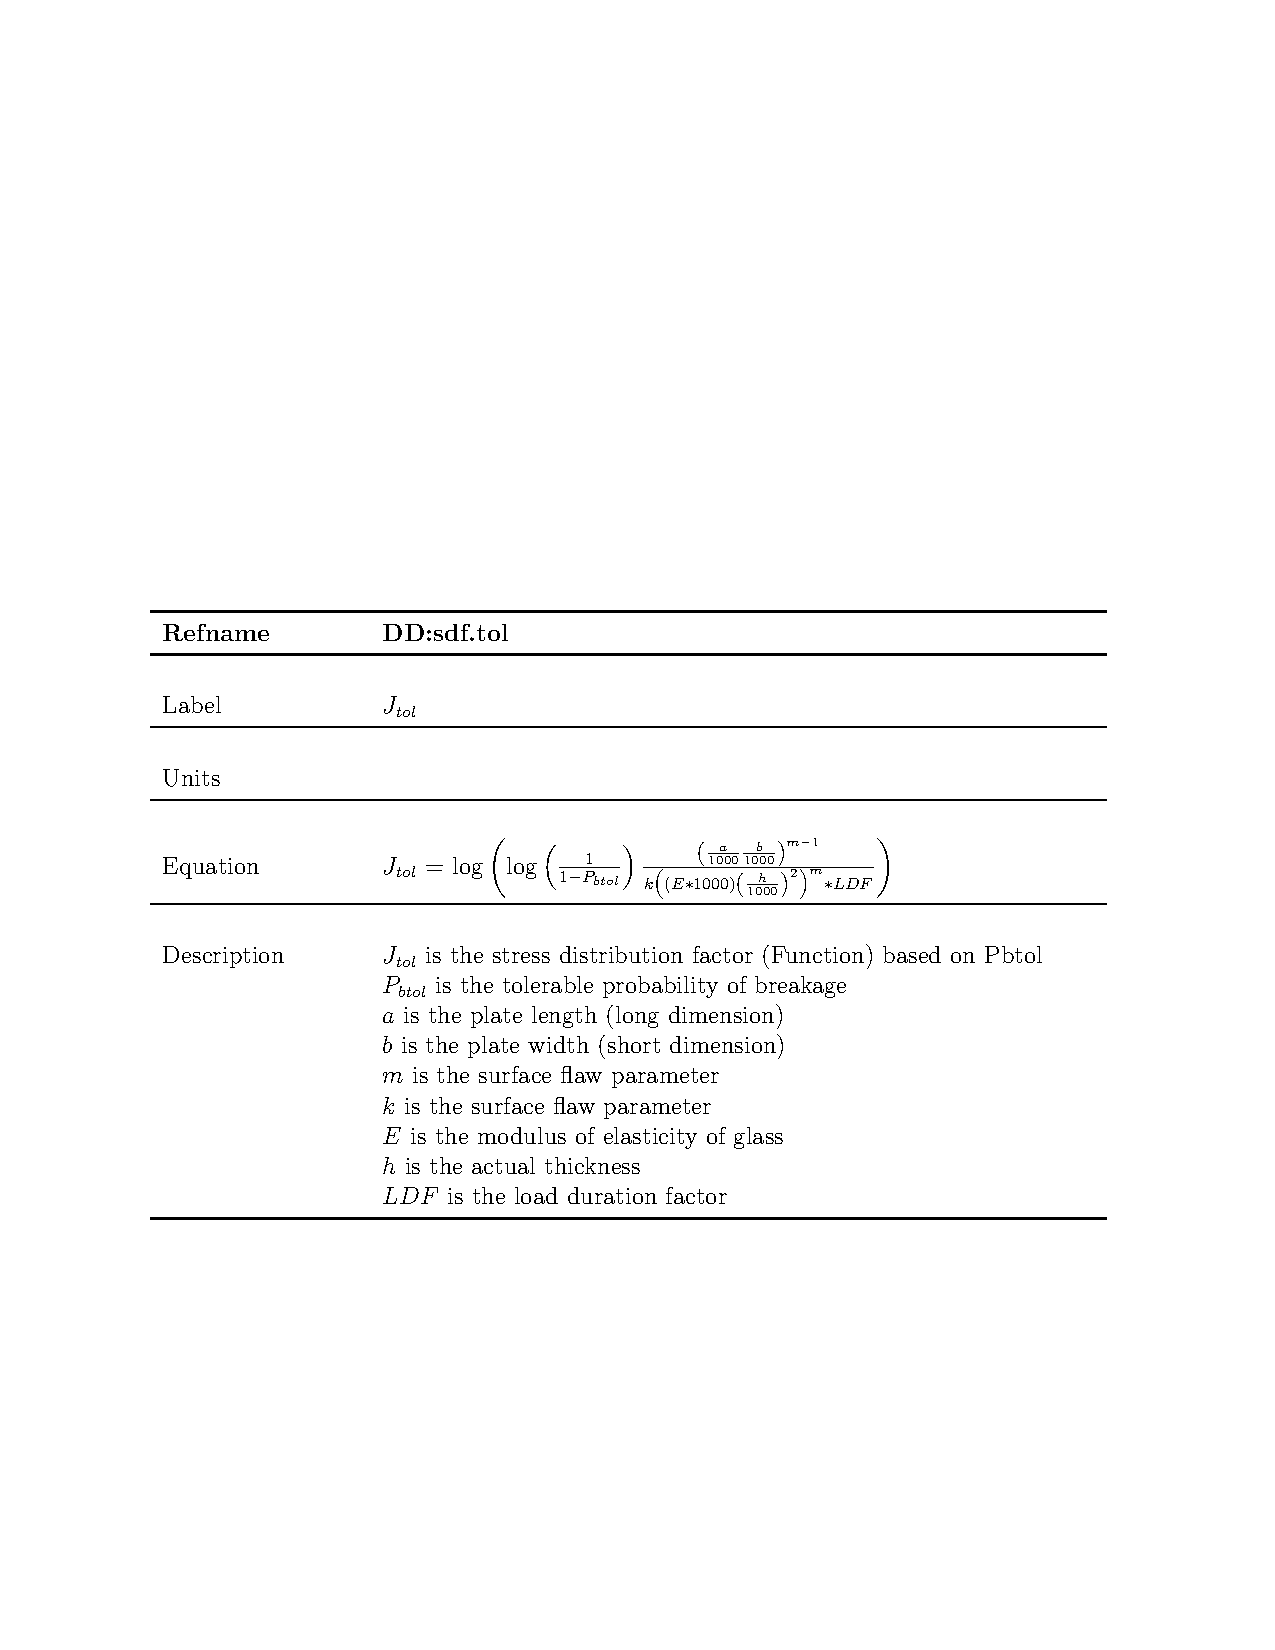
\includegraphics[width=0.45\textwidth]{./figures/Jtol_pdf.pdf}
\end{center}
\caption{$J_{\mbox{tol}}$ from GlassBR Requirements}
\label{Fig_Jtolpdf}
\end{figure}

- figure comes from tex generated by Drasil.  Can also generate html.  This
figure is part of the documentation of the requirements.  Eventually need code
to calculate Jtol.  Can generate code like in the next figure. \wss{this needs
  to be fit into one column}

\begin{figure}[htpb]
\begin{lstlisting} 
def calc_j_tol(inparams):
    j_tol = math.log((math.log(1.0/(1.0 - inparams.pbtol))) 
* ((((inparams.a / 1000.0) * (inparams.b / 1000.0)) ** (inparams.m - 1.0)) / ((inparams.k * (((inparams.E * 1000.0) * ((inparams.h / 1000.0) ** 2.0)) ** inparams.m)) * inparams.ldf)))
    return j_tol
\end{lstlisting}
\caption{Python code to Calculate $J_{\mbox{tol}}$}
\label{Fig_JtolPython}
\end{figure}

- can also generate Java, Lua, etc.

- next show the source file in Drasil.  \wss{need to fit in one column}

\begin{figure}[htpb]
\begin{lstlisting} 
stressDistFac = makeVC "stressDistFac" (nounPhraseSP 
  $ "stress distribution" ++ " factor (Function)") cJ

sdf_tol = makeVC "sdf_tol" (nounPhraseSP $ 
  "stress distribution" ++
  " factor (Function) based on Pbtol") 
  (sub (stressDistFac ^. symbol) (Atomic "tol"))

tolStrDisFac_eq :: Expr
tolStrDisFac_eq = log (log ((1) / ((1) - (C pb_tol)))
  * ((Grouping (((C plate_len) / (1000)) * ((C plate_width) / (1000)))) :^
  ((C sflawParamM) - (1)) / ((C sflawParamK) *
  (Grouping (Grouping ((C mod_elas) * (1000)) *
  (square (Grouping ((C act_thick) / (1000))))
  )) :^ (C sflawParamM) * (C loadDF))))

tolStrDisFac :: QDefinition
tolStrDisFac = mkDataDef sdf_tol tolStrDisFac_eq
\end{lstlisting}
\caption{Drasil (Haskell) code for $J_{\mbox{tol}}$ Knowledge}
\label{Fig_JtolDrasil}
\end{figure}

Now notice a mistake in code - shouldn't divide by 1000 - redo - fixes the
mistake everywhere

\begin{figure}[htpb]
\begin{lstlisting} 
tolStrDisFac_eq :: Expr
tolStrDisFac_eq = log (log ((1) / ((1) - (C pb_tol)))
  * ((Grouping ((C plate_len) * (C plate_width))) :^
  ((C sflawParamM) - (1)) / ((C sflawParamK) *
  (Grouping ((C mod_elas) * (square (C act_thick)))) :^ (C sflawParamM) * (C loadDF))))
\end{lstlisting}
\caption{Modified Drasil (Haskell) code for $J_{\mbox{tol}}$}
\label{Fig_JtolDrasil_fix}
\end{figure}

All of the knowledge on GlassBR can be put together to generate the software
requirements specification.  Can point to a figure showing the table of contents
for the SRS.  Explain that it can be generated in tex (pdf) or html.

\begin{figure}[htpb]
\begin{center}
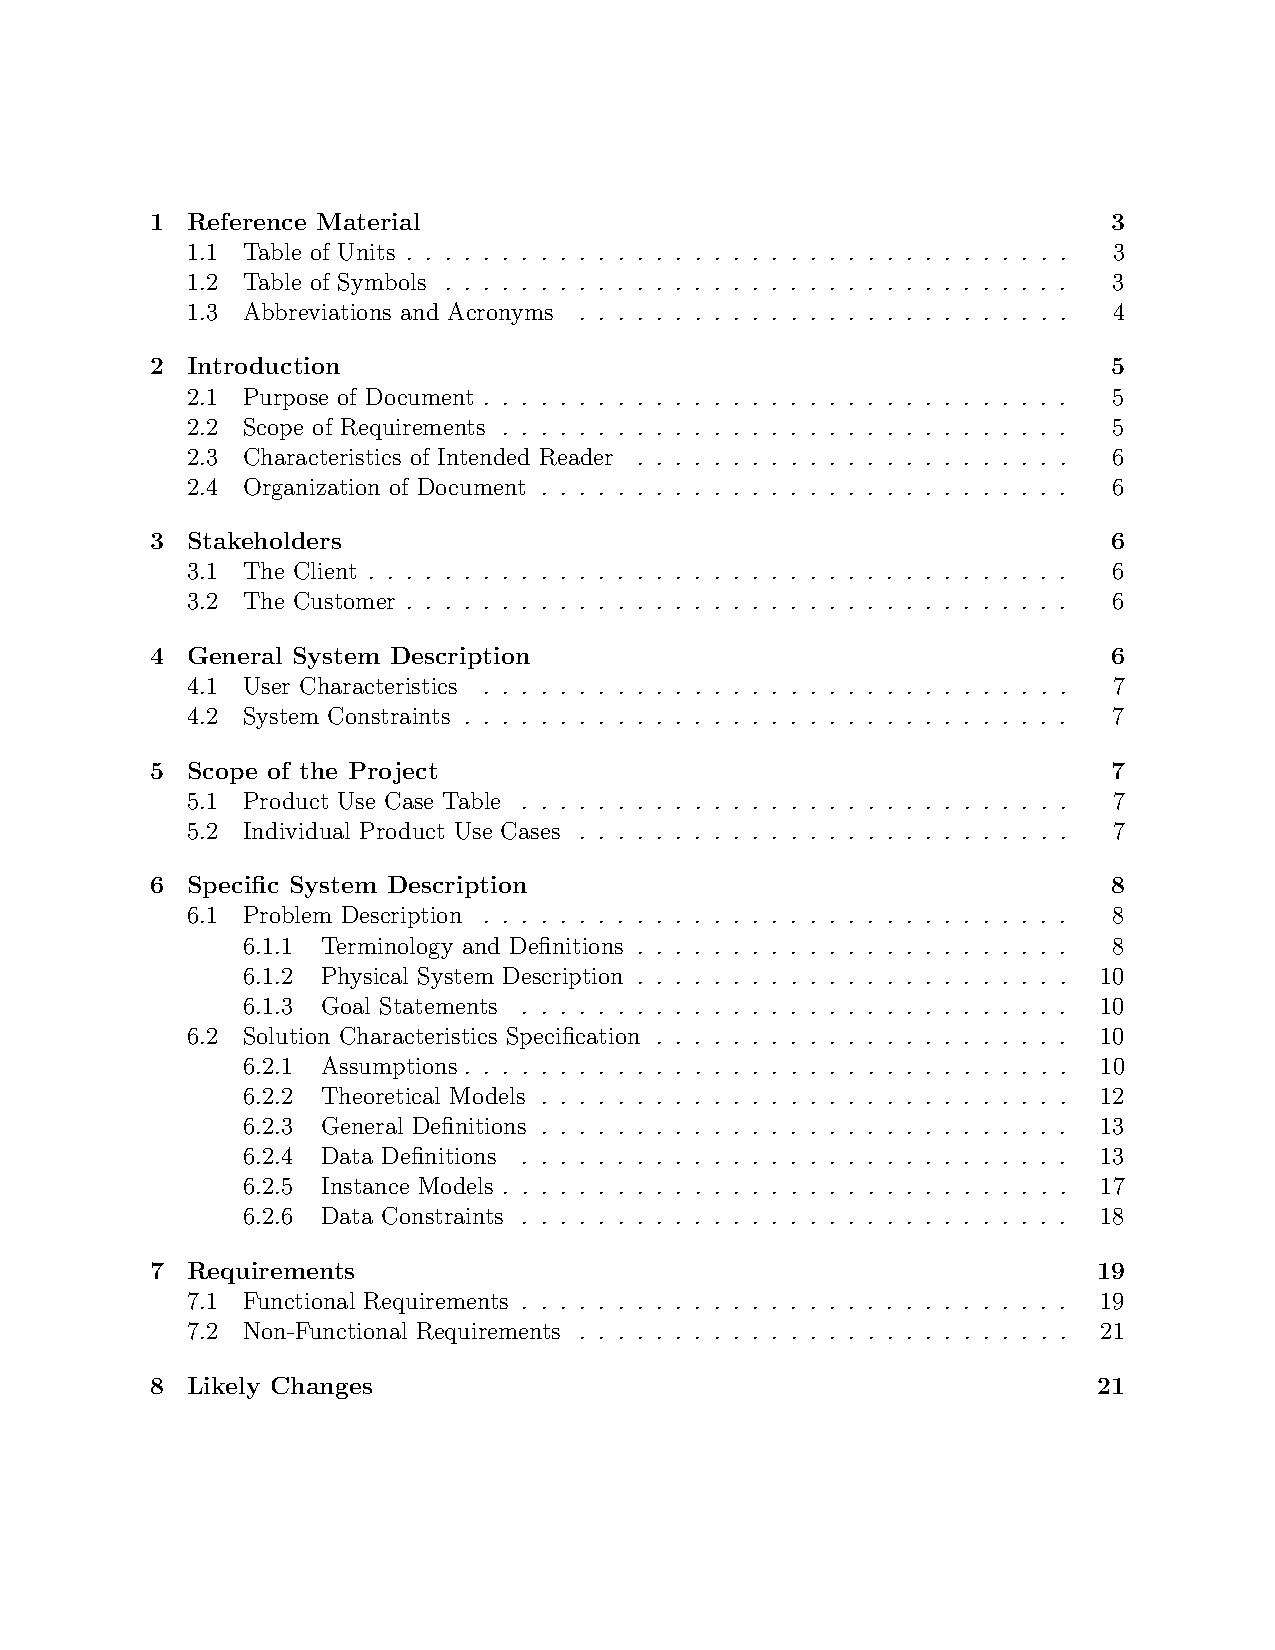
\includegraphics[scale=0.45]{./figures/TofC.pdf}
\end{center}
\caption{Table of Contents for Generated SRS for GlassBR}
\label{Fig_JtolDrasil}
\end{figure}

Part of SRS is automatically generated traceability information between
definitions, assumptions, theories and instanced models.

\begin{figure}[htpb]
\begin{center}
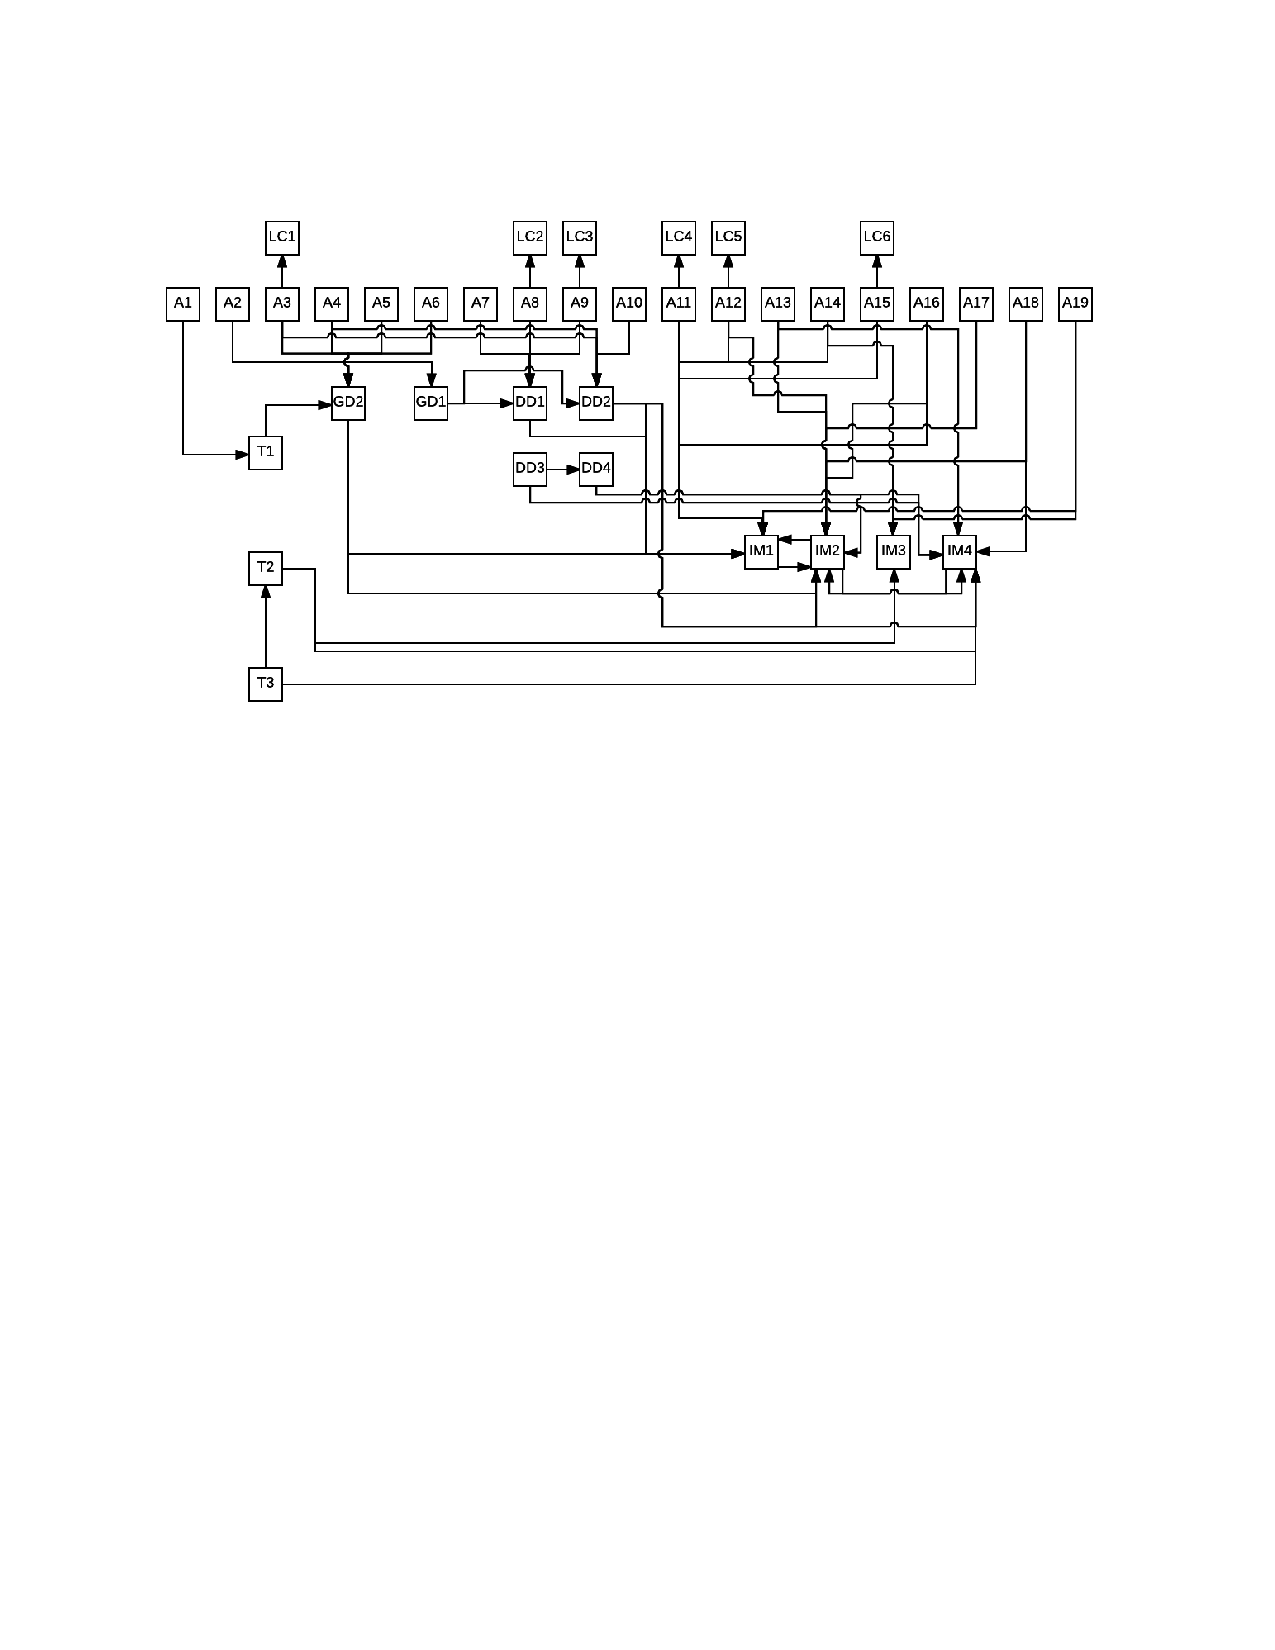
\includegraphics[scale=0.45]{./figures/TraceGraph.pdf}
\end{center}
\caption{Traceability Graph}
\label{Fig_JtolDrasil}
\end{figure}

\section{Quality Improvements} \label{SecQuality}

\subsection{Certifiability}

\begin{table} 
\centering
\caption{Constraints on quantities Used To Verify Inputs}
\begin{tabular}{c c r c } 
\toprule
\textbf{Var} & \textbf{Constraints} & \textbf{Typical Value} & \textbf{Uncertainty}\\ \midrule
$L$ & $L > 0$ & 1.5 m & 10\% \\ 
$\rho_P$ & $\rho_P > 0$	& 1007 kg/m$^3$	& 10\% \\
\bottomrule
\end{tabular}
\label{tab:pcm}
\end{table}

\begin{equation*}
E_W = \int_{0}^{t} h_C A_C (T_C - T_W(t)) dt - \int_{0}^{t} h_P A_P (T_W(t) - T_P(t)) dt
\end{equation*}

\begin{itemize}
\item \emph{If wrong, wrong everywhere}
\item Sanity checks captured and reused
\item Generate guards against invalid input
\item Generate test cases
\item Generate view suitable for inspection
\item Traceability for verification of change
\end{itemize}

\subsection{Reusability}

\begin{itemize}
\item De-embed knowledge
\item Reuse throughout document
\begin{itemize}
\item Units
\item Symbols
\item Descriptions
\item Traceability information
\end{itemize}
\item Reuse between documents
\begin{itemize}
\item SRS
\item MIS
\item Code
\item Test cases
\end{itemize}
\item Reuse between projects
\begin{itemize}
\item Knowledge reuse
\item A family of related models, or reuse of pieces
\item Conservation of thermal energy
\item Interpolation
\item Etc.
\end{itemize}
\end{itemize}

\subsection{Reproducibility}

\begin{itemize}
\item Usual emphasis is on reproducing code execution
\item However, \cite{IonescuAndJansson2013} show reproducibility challenges due to
undocumented:
\begin{itemize}
\item Assumptions
\item Modifications
\item Hacks
\end{itemize}
\item Shouldn't it be easier to independently replicate the work of others?
\item Require theory, assumptions, equations, etc.
\item Drasil can potentially check for completeness and consistency
\end{itemize}

\section{Future Work}

\section{Concluding Remarks}

\section{Acknowledgments}

The assistance of McMaster University's Dr.\ Manuel Campidelli, Dr.\ Wael and
Dr.\ Michael Tait with the GlassBR example is greatly appreciated.

\bibliographystyle{ACM-Reference-Format}
\bibliography{SzymczakEtAl2017} 

\end{document}